%%%%%%%%%%%%%%%%%%%%%%%%%%%%%%%%%%%%%%%%%%%%%%%%%%%%%%%%%%%%%%%%%%%%%%%%%%%%%%%%
%2345678901234567890123456789012345678901234567890123456789012345678901234567890
%        1         2         3         4         5         6         7         8

%\documentclass[letterpaper, 10 pt,noend]{article}  % Comment this line out if you need a4paper

\documentclass[letterpaper, 10pt, conference]{ieeeconf}      % Use this line for a4 paper

%\IEEEoverridecommandlockouts                              % This command is only needed if 
                                                          % you want to use the \thanks command

%\overrideIEEEmargins                                      % Needed to meet printer requirements.

% See the \addtolength command later in the file to balance the column lengths
% on the last page of the document

% numbers option provides compact numerical references in the text. 

\usepackage{float}
\usepackage[hidelinks, bookmarks=true]{hyperref}
\usepackage[font=small,labelfont=bf]{caption}

% The following packages can be found on http:\\www.ctan.org
\usepackage{graphics} % for pdf, bitmapped graphics files
\usepackage{epsfig} % for postscript graphics files
\usepackage{amsmath} % assumes amsmath package installed
\usepackage{amssymb}  % assumes amsmath package installed
\usepackage{listings}
\usepackage{graphicx,float,wrapfig}
\usepackage{subfig}
\usepackage{algpseudocode}
\usepackage{algorithm}
\usepackage{mathtools}
\usepackage{cite}
\usepackage{color}
\usepackage{comment}
\usepackage[usenames,dvipsnames,svgnames,table]{xcolor}
%\usepackage[inline,shortlabels]{enumitem}

\graphicspath{{pics/}}

%% Define symbols and special formats for texts
\DeclareMathOperator{\F}{\rotatebox[origin=c]{45}{$\Box$}}
\DeclareMathOperator{\G}{\Box}
\DeclareMathOperator{\X}{\bigcirc}
\DeclareMathOperator{\Cox}{\scalebox{0.8}{$\F$}\hspace{-9.3pt}\bigcirc}
\newcommand{\NN}{\mathbb{N}}
\newcommand{\FALSE}{\mathbf{false}}
\newcommand{\TRUE}{\mathbf{true}}
\newcommand{\TODO}[1]{{\color{red}#1}}

\title{\LARGE \bf MandM: Manipulation and Modular Robots with Baxter}


\author{Scott Hamill, Gangyuan Jing, Kai Weng Wong% <-this % stops a space
}


\begin{document}


\maketitle
\thispagestyle{empty}
\pagestyle{empty}

% add our sections here
\section{Introduction and Background}


Creating robot controllers by combining high-level task planning with low level motion planning has been a topic of recent interest \cite{HKG2009,Belta2008,Bhatia2011,Dornhege2009,Erdem2011,Tom2014,Srivastava2014}.
The integration of discrete task reasoning and motion planning allows users to specify complex robot behaviors and tasks from a high-level perspective while satisfying low level motion constraints.

Past research has shown promising results on controller synthesis with formal methods \cite{HKG2009,Belta2008,Bhatia2011,Wongpiromsarn,Maly,Vasile}.
Recent research has addressed controller synthesis using formal methods, specifying tasks and behaviors in a formal language such as Linear Temporal Logic (LTL) \cite{HKG2009,Belta2008,Bhatia2011,Dornhege2009,Erdem2011,Tom2014,Srivastava2014}.
Controllers synthesized in this manner are correct-by-construction, thereby providing guarantees on the behavior of the robot.
These algorithms typically abstract the robot system and environment by discretizing the workspace.
This technique works well for mobile robot systems, but discretizations for manipulation systems are typically intractable due to combinatorial blow-up of the state space.

Formal methods have previously been applied to controller synthesis for manipulation \cite{Dornhege2009,Erdem2011,Tom2014,Srivastava2014,CambonAG09,KaelblingL11,PlakuH10,HeLKV15}.
Most of these works utilize AI based planners for high-level task planning and low-level motion planners for finding feasible robot trajectories \cite{Nau,Hoffmann01}.
While these frameworks allow users to specify high-level behaviors and task specifications, the resulting behaviors are non-reactive in that the robot behavior does not depend on the state of the environment.

This work addresses synthesizing correct-by-construction controllers for a manipulation task from a high-level behavioral specification.
This framework provides three main contributions: a high-level {\it task planner} for determining sequences of high-level actions, a {\it trajectory planner} for finding and executing feasible manipulator motions, and an {\it action planner} for performing precise manipulator motion and actuation.
This framework is is demonstrated on a Baxter robot (Rethink Robotics) assembling a series of modular robot components into a pre-defined configuration. 


\begin{comment}
With the development of hardware and software of robots,
There is an increasing interest in combining high-level task planning
with low-level motion planning when creating robot controllers \cite{HKG2009,Belta2008,Bhatia2011,Dornhege2009,Erdem2011,Tom2014,Srivastava2014}.
While integrating tasking and motion planning enables users to specify complex robot tasks from a high-level perspective,
combining discrete task reasoning with continuous motion planning brings challenges to designing robot controllers.

Past research has shown promising results on controller synthesis with formal methods \cite{HKG2009,Belta2008,Bhatia2011,Wongpiromsarn,Maly,Vasile}.
In these papers, robot tasks are expressed in formal language such as Linear Temporal Logic (LTL).
Controllers can be automatically synthesized from the task specification,
while providing guarantees on the correctness of robot behaviours.
These controller synthesis algorithms typically abstract robot systems and environment by discretizing the robot workspace,
in order to avoid the combinatorial blow up of the state space.
While the abstraction reduces the complexity of mobile systems,
the discretization is usually intractable for manipulation systems,
due to high degrees of freedom of manipulation tasks.

Many frameworks were developed on controller synthesis with formal methods for manipulation \cite{Dornhege2009,Erdem2011,Tom2014,Srivastava2014,CambonAG09,KaelblingL11,PlakuH10,HeLKV15}.
Most of these works utilize AI based planners for high-level task planning and low-level motion planners for finding feasible robot trajectories \cite{Nau,Hoffmann01}.
These frameworks allows user to control manipulation systems with high-level task specifications.
However, high-level planners used in these frameworks limit possible tasks to non-reactive,
i.e. the behavior of the robot does not depend on the state of the environment.

Moreover, formal methods are also used in robotics to generate controllers for coordination of a team of robots \cite{ChenDSB12,KaramanF08,GuoTD14,VasileB14}.
In these work, tasks are specified in Temporal Logic and controllers are automatically synthesized and distributed to each robot agent. 
However, little work has been done on task and motion planning for multi-agent manipulation system with formal method.

In this work, we are interested in developing a framework for automatically synthesizing correct-by-construction controllers
for multi-agent manipulation tasks expressed in Linear Temporal Logic. The framework consists of three main components:
a high-level \textit{task planner} for generating and distributing controllers to each agent,
a \textit{trajectory planner} for finding feasible path and moving each manipulator while avoiding collisions,
and and \textit{action planner} for creating precise motion and actuation for each manipulator.
The framework will be demonstrated with an experiment of two physical Baxter robots assembling a set of modular robots. 
\end{comment}

\section{Preliminaries}\label{prelim}

\paragraph{AprilTags} AprilTags are 2D barcodes developed for robotics applications by Ed Olson ~\cite{Olson11}. With an existing framework, the position and orientation of any AprilTag in a given image can be automatically detected. In this work we use this system to localize the position and orientation of modules.

\section{Problem Formulation and Overview}\label{pf}

\subsection{Problem Formulation}

Given a certain number of modular SMORES robots with randomized initial positions and orientations, assemble the robots into a goal configuration specified by the user.

\subsection{Project Overview}\label{overview}
In this work, we are interested in developing a framework for controlling a Baxter robot to automatically assemble a set of modular robots into a single configuration based on the user defined {\it configuration file}.
Moreover, we aim to provide guarantees for the behaviors of the robot to the user during the planning stage to avoid unexpected or unsafe behaviors.
Specifically, the frameworks includes the following main components:
\begin{itemize}
\item A high-level planner for parsing user defined {\it configuration file} and generate and execute an assembly plan. 
\item A trajectory planer that is capable of moving robot arms to any configuration with its workspace while avoiding collisions.
\item An action planner for creating precise and verified motion to control the end effector of each arm.
\end{itemize}
%\section{Overview}\label{overview}

% system diagram
\section{Task Planning}
The task planner in this work is based on the framework introduced in (\TODO{hadas paper}).
\begin{itemize}
\item Change specification language for multirobot
\item How to distribute tasks from a single automaton
\item How to deal with the situation when the trajectory planner returns not path?
\end{itemize}
\section{Trajectory Planning (Catherine)}

This component is divided into two subsections:
\begin{enumerate}%[label=\thesection.\arabic*]
\item Trajectory Planner for robot arm trajectory planning, and
\item Trajectory Executor for robot arm trajectory execution.
\end{enumerate}

\subsection{Trajectory Planner}

During execution, the task planner requests the path planner to create trajectory plans for one or more robot arms. The planner aims to find a plan that (i) each arm starts at its initial configuration, and (ii) each arm ends with each robot end effector within a certain radius from the final desired workspace position. If the planner finds a plan, it returns the joint-space trajectory for each arm. If the planning exceeds the time limit, then the planner aborts and returns no trajectories. 

There are a variety of path planning algorithms developed in the community~\cite{DBLP:books/daglib/0016830} and some algorithms are adapted for finding robot arm trajectories. 
Researchers have proposed sampling-based approaches with probabilistic completeness such as the Rapidly-Exploring Random Tree (RRT) algorithm ~\cite{VahrenkampBAKD09} to find trajectories for robot arms. Others have used Probabilistic RoadMaps (PRM) that work with high-dimensional spaces~\cite{KavrakiSLO96} but the algorithm requires pre-computation of the roadmap and no dynamic obstacles in the environment. In this project, we will not conduct pre-processing and the other arms can become obstacles so we are using RRT to find trajectories for the robot arms.

First, we plan to try two different RRT approaches and compare their performance. With RRT, there are still multiple ways to generate a trajectory plan.
One of them is to generate trajectory plan synchronously.
For example, if there are four arms available for a task, or two Baxters, then the planning could be synchronous, i.e, we plan all the arms at the same time and each node in RRT stores the joint information of the four arms. With each arm having 7 degrees of freedom (DoF), a synchronous planning has up to 28 degrees of freedom.
With this approach, assuming the workspace has no other obstacles, collision avoidance with the other arms is taken care of during the planning phase so it is unnecessary during trajectory execution.  
The trade off of synchronous planning is that one arm may wait for the others even though its trajectory is found.

Alternatively, another way would be to first create a plan each arm separately and assign priorities to each arm. An arm then replans only when its trajectory intersects with the plan of another arm with a higher priority. Compared with the synchronous approach, each planning contains 7 degrees of freedom but re-plannings of trajectory can go up to (n-1) times, with n being the number of arms. 

Second, we plan to create our own version of RRT planner and also utilize off-the-shelf library with RRT such as the Open Motion Planning library (OMPL)~\cite{sucan2012the-open-motion-planning-library} to find out the one with better performance.
Compared with creating our own RRT planner, OMPL has lots of planning algorithms available, but most examples of OMPL work with single robot or arm and planning for multiple arms simultaneously with OMPL may be unfeasible. We plan to learn more about OMPL and then decide if we are creating our own RRT planner or we are using OMPL to build our planner.

Finally, RRT is only a template for planning and we need to complete the template with ways to propagate a trajectory and smoothen the resulting trajectory. 
During the planning phrase, we plan to optimize the final trajectory by reducing the difference in joint angles between two nodes in the RRT tree. We use inverse kinematics find robot joint angles given a desired location of the end effector.


%To conduct a path planning of the robot arms, the planner takes in:

%\begin{itemize}
%\item the number of arms we are planning, 
%\item the starting joint configurations of each arm, and
%\item the final workspace positions of robot end effectors.
%\end{itemize}

two-step planning


\subsection{Trajectory Executor}

Besides a trajectory planner, the person in charge of this component also creates a trajectory executor that executes any given trajectory.
Once the task planner receives a plan, it can invoke the trajectory executor to execute the path. The executor takes in a joint-space trajectory and notifies the task planner when it finishes the execution. The task planner then invokes planning by the action planner in the next section to conduct fine and accurate objects manipulation.

\section{Action Planning and Verification (Scott)}

The action planning process involves modeling the manipulator behavior and verifying a controller with respect to any safety conditions specified by the user.
The trajectory planner is responsible for executing a rough motion of the manipulator to some approximate pose near the final desired location of the end effector (EFF).
In the case of the modular robot assembly, the trajectory planner moves the modular robot component to be attached to a location near the final attachment EFF pose.
The task planner provides the desired translation of the EFF in the global reference frame (necessary for making the connection) to the action planner, which then executes the motion once it the controller has been verified.


\subsection{Continuous System Verification}
In order to avoid undesirable robot motions, the user specifies a set of unsafe states of the robot, $\varphi$, for a given action or motion of the manipulator.
For the case of modular robot assembly, the unsafe set is defined to be those poses of the end effector during an attachment motion that may result in a failed attachment or improper connection (magnet misalignment).
A given controller may be verified to cause the system remain within the safe set (no intersection with the unsafe set) by computing the set of all reachable states, $\textit{ReachSet}_{\mbox{\textit{H}}}$, from some initial condition ,$X_0 \subseteq X$.
However, the exact set of reachable states is difficult \cite{Henzinger:1995:WDH:225058.225162}, and an over approximation of the reachable set is instead computed.
The controller is verified if the over approximated set is contained within the set of states that satisfy the safety conditions, $\mbox{\textit{ReachSet}}_{\mbox{\textit{H}}} \subseteq \mbox{Sat}(\varphi)$.
The controller and motion are not verified if there is an intersection of the reachable states and the unsafe set, $\mbox{\textit{ReachSet}}_{\mbox{\textit{H}}} \cap \neg \mbox{Sat}(\varphi) \neq \emptyset$.
In the case where some intersection of the unsafe set and reachable set occurs, no conclusions may be drawn from the analysis as the reach set is an over approximation and re-planning of the manipulator (by the trajectory planner) is required.

This process is similar to the framework in \cite{6016596}, whereby the control architectures of an autonomous robotic surgery manipulator are verified for a puncturing tasks, whereby the EFF (puncturing instrument) is guaranteed to remain within some pose bounds.
In this work, the reachability tool Flow* \cite{Chen2013} is used to over approximate the system dynamics using Taylor Model flowpipes.
Flow* is capable of handling nonlinear systems, but as manipulators are highly nonlinear, the dynamics of the Baxter arms are linearized in an effort to increase computation speed. 


\subsection{Manipulator Modeling}
The dynamics of each of the Baxter arms can be represented as:
\begin{equation}
	\mathbf{M}(\underline{q})\ddot{\underline{q}} + \mathbf{C}(\underline{q},\underline{\dot{q}})\dot{\underline{q}} + \mathbf{G}(\underline{q}) = \underline{T}_{eff} + \underline{T}_{in}
\end{equation}
Where $\mathbf{M}$ and $\mathbf{C}$ represent the inertial effects, $\mathbf{G}$ represents joint torques due to gravity, $\underline{T}_{EFF}$ represents the joint torques due to EFF load, and $\underline{T}_{in}$ represents the input joint torques.
In this case, linearizing the arm dynamics involves evaluating the nonlinear $\mathbf{M}$, $\mathbf{C}$, and $\mathbf{G}$ matrices for a given arm configuration.
As the action planner only executes arm motions for small EFF motions (and subsequently small changes in joint angle) it is assumed that these matrices remain constant for the duration of the arm motion executed by the action planner.
It should be noted that Coriolis effects, $\mathbf{C}$, are ignored due to the small motions of the arm.


\subsection{ROS Action Server and Code Diagram}
The action planner, comprised of the reachability analysis, controller verification, and joint torque controller execution are implemented as an action server in ROS.
The code block diagram is shown in figure Fig. \ref{fig:actionPlannerFlow}.
The action server, when called by the task planner when a connection need to be performed, polls the current state of the arm holding the module to be attached, computes the linearized matrices, generates a Flow* file, performs the reachability computation for the given feedback controller, then executes the motion.
The server creates an instance of Matlab when launched, which is then used for the kinematics computations and controller design.
The kinematics computations and linear model generation are done using the Matlab Robotics Toolbox \cite{Corke11a}.

\begin{figure}[h]
	\includegraphics[width = 8 cm]{action_server_2.png}
	\caption{Action Planner Module}
	\label{fig:actionPlannerFlow}
\end{figure}


\subsection{Difficulties with Baxter Joint Torque Control}
Initially, the controller used in the action planner server was a linear quadratic regulator (LQR) controller computed by Matlab.
The LQR controller provided feedback joint torques while a static input was added to counteract gravitational effects ($\mathbf{G}$ torques).
However, this controller, when implemented on the Baxter platform, resulted in erratic arm motions despite satisfactory performance in the Baxter simulator.
The Baxter platform provides a ``zero-gravity'' mode of operation whereby the robot continually provides torques to each joint sufficient to counteract gravitational effects.
The LQR controller, when implemented in ``zero-gravity'' mode (without the added gravitational torque compensation), resulted in arm ``drift,'' whereby the arm would slowly diverge from the initial condition.
Increasing the control effort did not improve the ability of the LQR controller to overcome the perceived arm ``drift.''
When the LQR controller was implemented with the ``zero-gravity'' mode disabled (which included the gravitational torque compensation), the resulting arm motion was wildly erratic.
Operating with the ``zero-gravity'' mode disabled is not recommended.

The controller implemented in the final version of the action planner server (torque control) is a PD controller.
The robot has pre-defined joint spring and damping coefficients that can be called for PD joint torque control.
This controller (when used in ``zero-gravity'' mode) results in stable arm motion, both in simulation and on the physical robot.
However, the default spring and damping values result in significant arm oscillations when the robot is moving from one configuration to another.
As oscillations are undesirable when connecting modular components, the damping values are increased.
It should be noted that both the spring and damping coefficient values are passed in to the action planner server when called and, as such, may be altered at runtime by the task planner.

\subsection{Verified Motion Example}
The results of the execution of a simple motion command on the left arm by the action planner are shown in Figures \ref{fig:effX},\ref{fig:effY}, and \ref{fig:effZ}.
In this example, the input desired EFF motion is appx. 10 cm in the negative z direction (toward the ground) in the Baxter global reference frame, starting in the neutral arm position.
The values plotted are with respect to the starting $x/y/z$ EFF position.

\begin{figure}[h]
	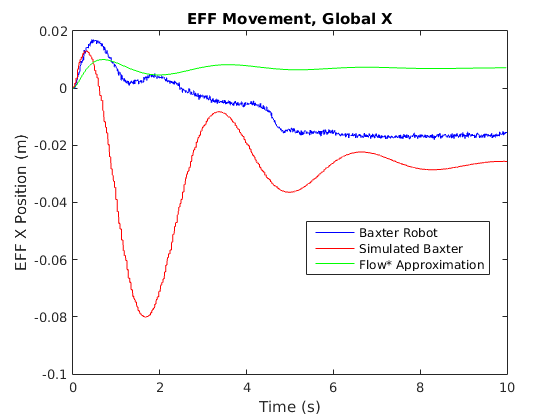
\includegraphics[width = 8 cm]{effx_example.png}
	\caption{Example Action Planner Execution, EFF $X$ motion}
	\label{fig:effX}
\end{figure}

\begin{figure}[h]
	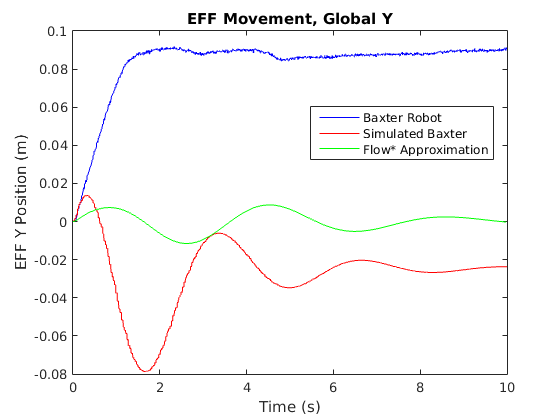
\includegraphics[width = 8 cm]{effy_example.png}
	\caption{Example Action Planner Execution, EFF $Y$ motion}
	\label{fig:effY}
\end{figure}

\begin{figure}[h]
	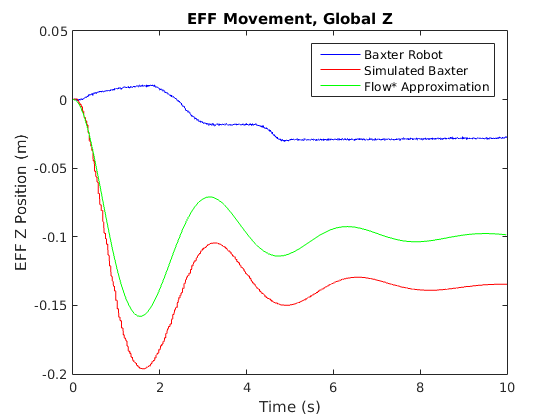
\includegraphics[width = 8 cm]{effz_example.png}
	\caption{Example Action Planner Execution, EFF $Z$ motion}
	\label{fig:effZ}
\end{figure}

The Flow* approximations, shown in green, show the computed reachable set for each EFF position variable $(x,y,z)$ as a function of time.
The range of the reachable set are small at each time step as the initial conditions for the computation are scalar values rather than a range.
Given a range of initial conditions (representing, for example, error in the measured joint angles) the computed reachable sets would show a greater range of values - the green lines wold appear more like funnels showing the over approximated upper and lower bounds for the variables.
The reachable sets shown are computed with scalar initial conditions for clarity.

The reachable sets computed from the linear model predict small deviations (< 2 cm) of the $x$ and $y$ EFF values during the motion and show the $z$ value converging to the desired value of -0.1, albeit with some oscillation.
Despite the near 5 cm overshoot in the $z$ direction predicted by the linear model, the small predicted $x$ and $y$ deviations may be sufficient for a successfully attaching a module.
However, the EFF motions recorded in the Baxter simulator and physical robot clearly do not agree with the predicted motions.
The data from the simulated Baxter robot shows significantly increased oscillations and the data from the physical robot shows stiff, heavily damped motions.
The motions of the physical robot during the execution of the action planner were observed to be stiff, jerky, and unrepeatable, likely due to significant, asymmetric friction in the arm joints.
As such, the output of the reachable set computation is not valid for determining the safety of a given controller.

\subsection{First Order Joint Control}
A first order (joint speed) controller was implemented in an effort to avoid the erratic behavior of the LQR and PD joint torque controllers.
Using the global reference frame Jacobian computed in the Matlab Robotics Toolbox, the required joint velocities are computed for a desired end effector translation.
This controller was used for the demonstration examples.









\begin{comment}
The action planning stage of the assembly process is broken down into two parts: modeling the manipulator behavior as a hybrid system and verifying safety conditions of the end effector motions (making sure that undesirable motions do not occur).

\subsection{Hybrid system modeling}
The trajectory planner discussed in the previous section is responsible for moving each arm (trajectory execution) to within some bound of the final desired end effector position (determined by the task planner) for either (i) grasping or (ii) component alignment. 
The trajectory planner provides to the action planner the final positions of the end effectors with respect to the appropriate blocks for (i) grasping, or (ii) alignment at attachment.
In either case, it is beneficial to avoid damaging a robot module or failing to complete a grasp or attachment due to position and alignment errors.
For the proposed scenario of assembling modular robotic components, we implement a system similar to a framework \cite{6016596} developed to address the verification of control architectures for autonomous robotic surgery manipulation tasks with respect to various safety conditions, denoted as $\varphi$, such as avoiding end effector misalignment or excessive force application.

In the previously mentioned framework, the system is modeled as a hybrid automaton \cite{Alur1993}, composed of discrete states (tasks/behaviors) and continuous dynamics associated with each state or behavior.
In our case of modular robot assembly, each state consists of \textit{fast approach}, which is handled by the trajectory planner, and \textit{slow approach}, \textit{alignment}, \textit{grasping}, and \textit{connecting}, handled by the action planner. 
Each state also contains a controller, a set of invariants (conditions required to be true while the automaton is in that state), and a set of guards (conditions that must be true in order for a state transition to take place).

\subsection{Verification of Behaviors}
In order to verify that the safety conditions $\varphi$ are satisfied for the discrete state controllers, the reachable set of the system $\textit{ReachSet}_{\mbox{\textit{H}}}$, which is the set of all reachable states from some initial condition, $X_0$, can be compared to the set of states for which the safety properties are not satisfied, $\neg \mbox{Sat}(\varphi)$.
However, computing the exact set of reachable states is difficult \cite{Henzinger:1995:WDH:225058.225162} and approximations may be used instead.
In this case, a reachability tool (e.g. \textit{SpaceEx}~\cite{rehseGDCRLRGDM11}), which computes approximate reachable sets given the system dynamics and controllers, can be used to over-approximate the reachable set of the hybrid system $\textit{ReachSet}_{\mbox{\textit{H}}}$ such that $\mbox{\textit{ReachSet}}_{\mbox{\textit{H}}} \supseteq \mbox{Sat}(\varphi)$, where $\mbox{Sat}(\varphi)$ is the set of states that satisfies $\varphi$.
If $\mbox{\textit{ReachSet}}_{\mbox{\textit{H}}}$ does not intersect with the set of states for which the safety conditions $\varphi$ is not satisfied, $\mbox{\textit{ReachSet}}_{\mbox{\textit{H}}} \cap \neg \mbox{Sat}(\varphi) = \emptyset$, the safety of the system is verified.

In the case that $\mbox{\textit{ReachSet}}_{\mbox{\textit{H}}} \cap \neg \mbox{Sat}(\varphi) \neq \emptyset$, the inconclusive nature of the system is communicated to the trajectory planner and the system will either (i) re-plan the arm motions or (ii) adjust the boundaries specified in the safety conditions, $\varphi$ and recompute the system reachability.

\end{comment}


\section{Experiment}

We conducted an experiment of our system with a Rethink Baxter robot and six wooden modules with AprilTags on them. For sensing and localization of the modules, we used the camera on Baxter's left hand and an external Kinect. In this experiment, we started from some random location of the six modules (Fig.~\ref{fig:initConfig}) and tried to form a snake configuration with the six modules (Fig.~\ref{fig:finalConfig}).
The link to a video of the experiment is \url{https://youtu.be/OXdHslVxjws}. 

\begin{figure}[ht!]%[H]
\centering
\subfloat[Inital position of the modules]{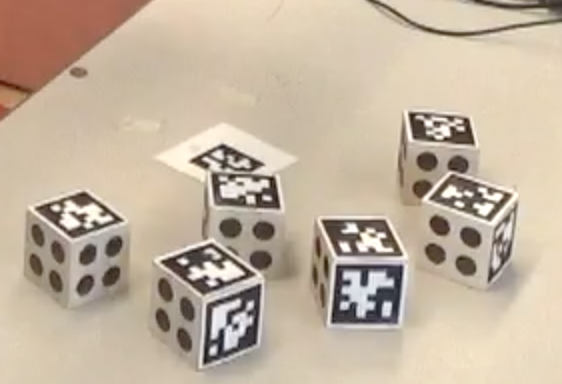
\includegraphics[width=0.45\columnwidth]{pics/init_module_location.png}\label{fig:initConfig}}
\quad
\subfloat[Final module configuration]{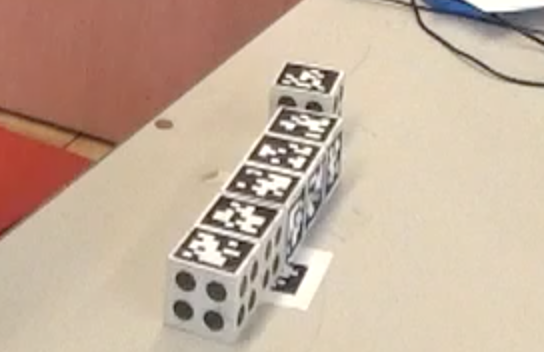
\includegraphics[width=0.45\columnwidth]{pics/snake_modules.png}\label{fig:finalConfig}}\\
\caption{Final Module Configuration}
\end{figure}

In this experiment, our system was able to recover from grasping failure and our system continued to finish the assembly with the instructions from the high-level planner. As shown in Table~\ref{table:result}, out of the five connections between the modules, our system successfully performed 3 connections: connected the third, the fourth and fifth module to the assembly. Our system failed to connect the second module to the first one due to misalignment and it also failed to connect the last module to the assembly due to too small of a motion. 


%\begin{center}
\begin{table}[h]
\caption{Connection Result of Modules} %F for Failed and S for Succeeded}
\begin{tabular}{|c |c |c |c |c |c|}
\hline
 Connection &  1-2 & 2-3 & 3-4 & 4-5 & 5-6 \\\hline 
  Result  & failed & succeeded & succeeded & succeeded & failed \\\hline  
\end{tabular}\label{table:result}
\end{table}
%\end{center}

In the future, we will improve the fine adjustment to connect the modules. We also want to conduct synthesis of the trajectory planner. We will use the right arm to localize and manipulate the modules. We plan to attempt more complex configuration to showcase the capabilities of our system.




\bibliographystyle{plain}
\bibliography{ref}

\end{document}
